\section{Blockierende und nichtblockierende \acs{I/O}}
 Ein nicht-blockierendes I/O-Modell ermöglicht die Verarbeitung von Befehlen bei zeitintensiven Berechnungen oder Datenbankabfragen ohne dass der Main-Thread der Anwendung blockiert wird. Es muss nicht auf das Ergebnis der Berechnung gewartet werden, bevor der nächste Befehl ausgeführt werden kann. Der Mechanismus kann beispielsweise mit Hilfe einer Event-Loop umgesetzt werden, die Vorgänge in sogenannten Worker-Threads auslagert und diesen jeweils eine Callback-Funktion übergibt. Die Funktion wird im Main-Thread aufgerufen, sobald der jeweilige Berechnungsvorgang beendet ist (siehe Abb. \ref{img:nonblocking}). Diese Technik nennt sich \acf{CPS} und wird im Kapitel \ref{CPS} am Beispiel von JavaScript erklärt.
\begin{figure}[H]
\centering
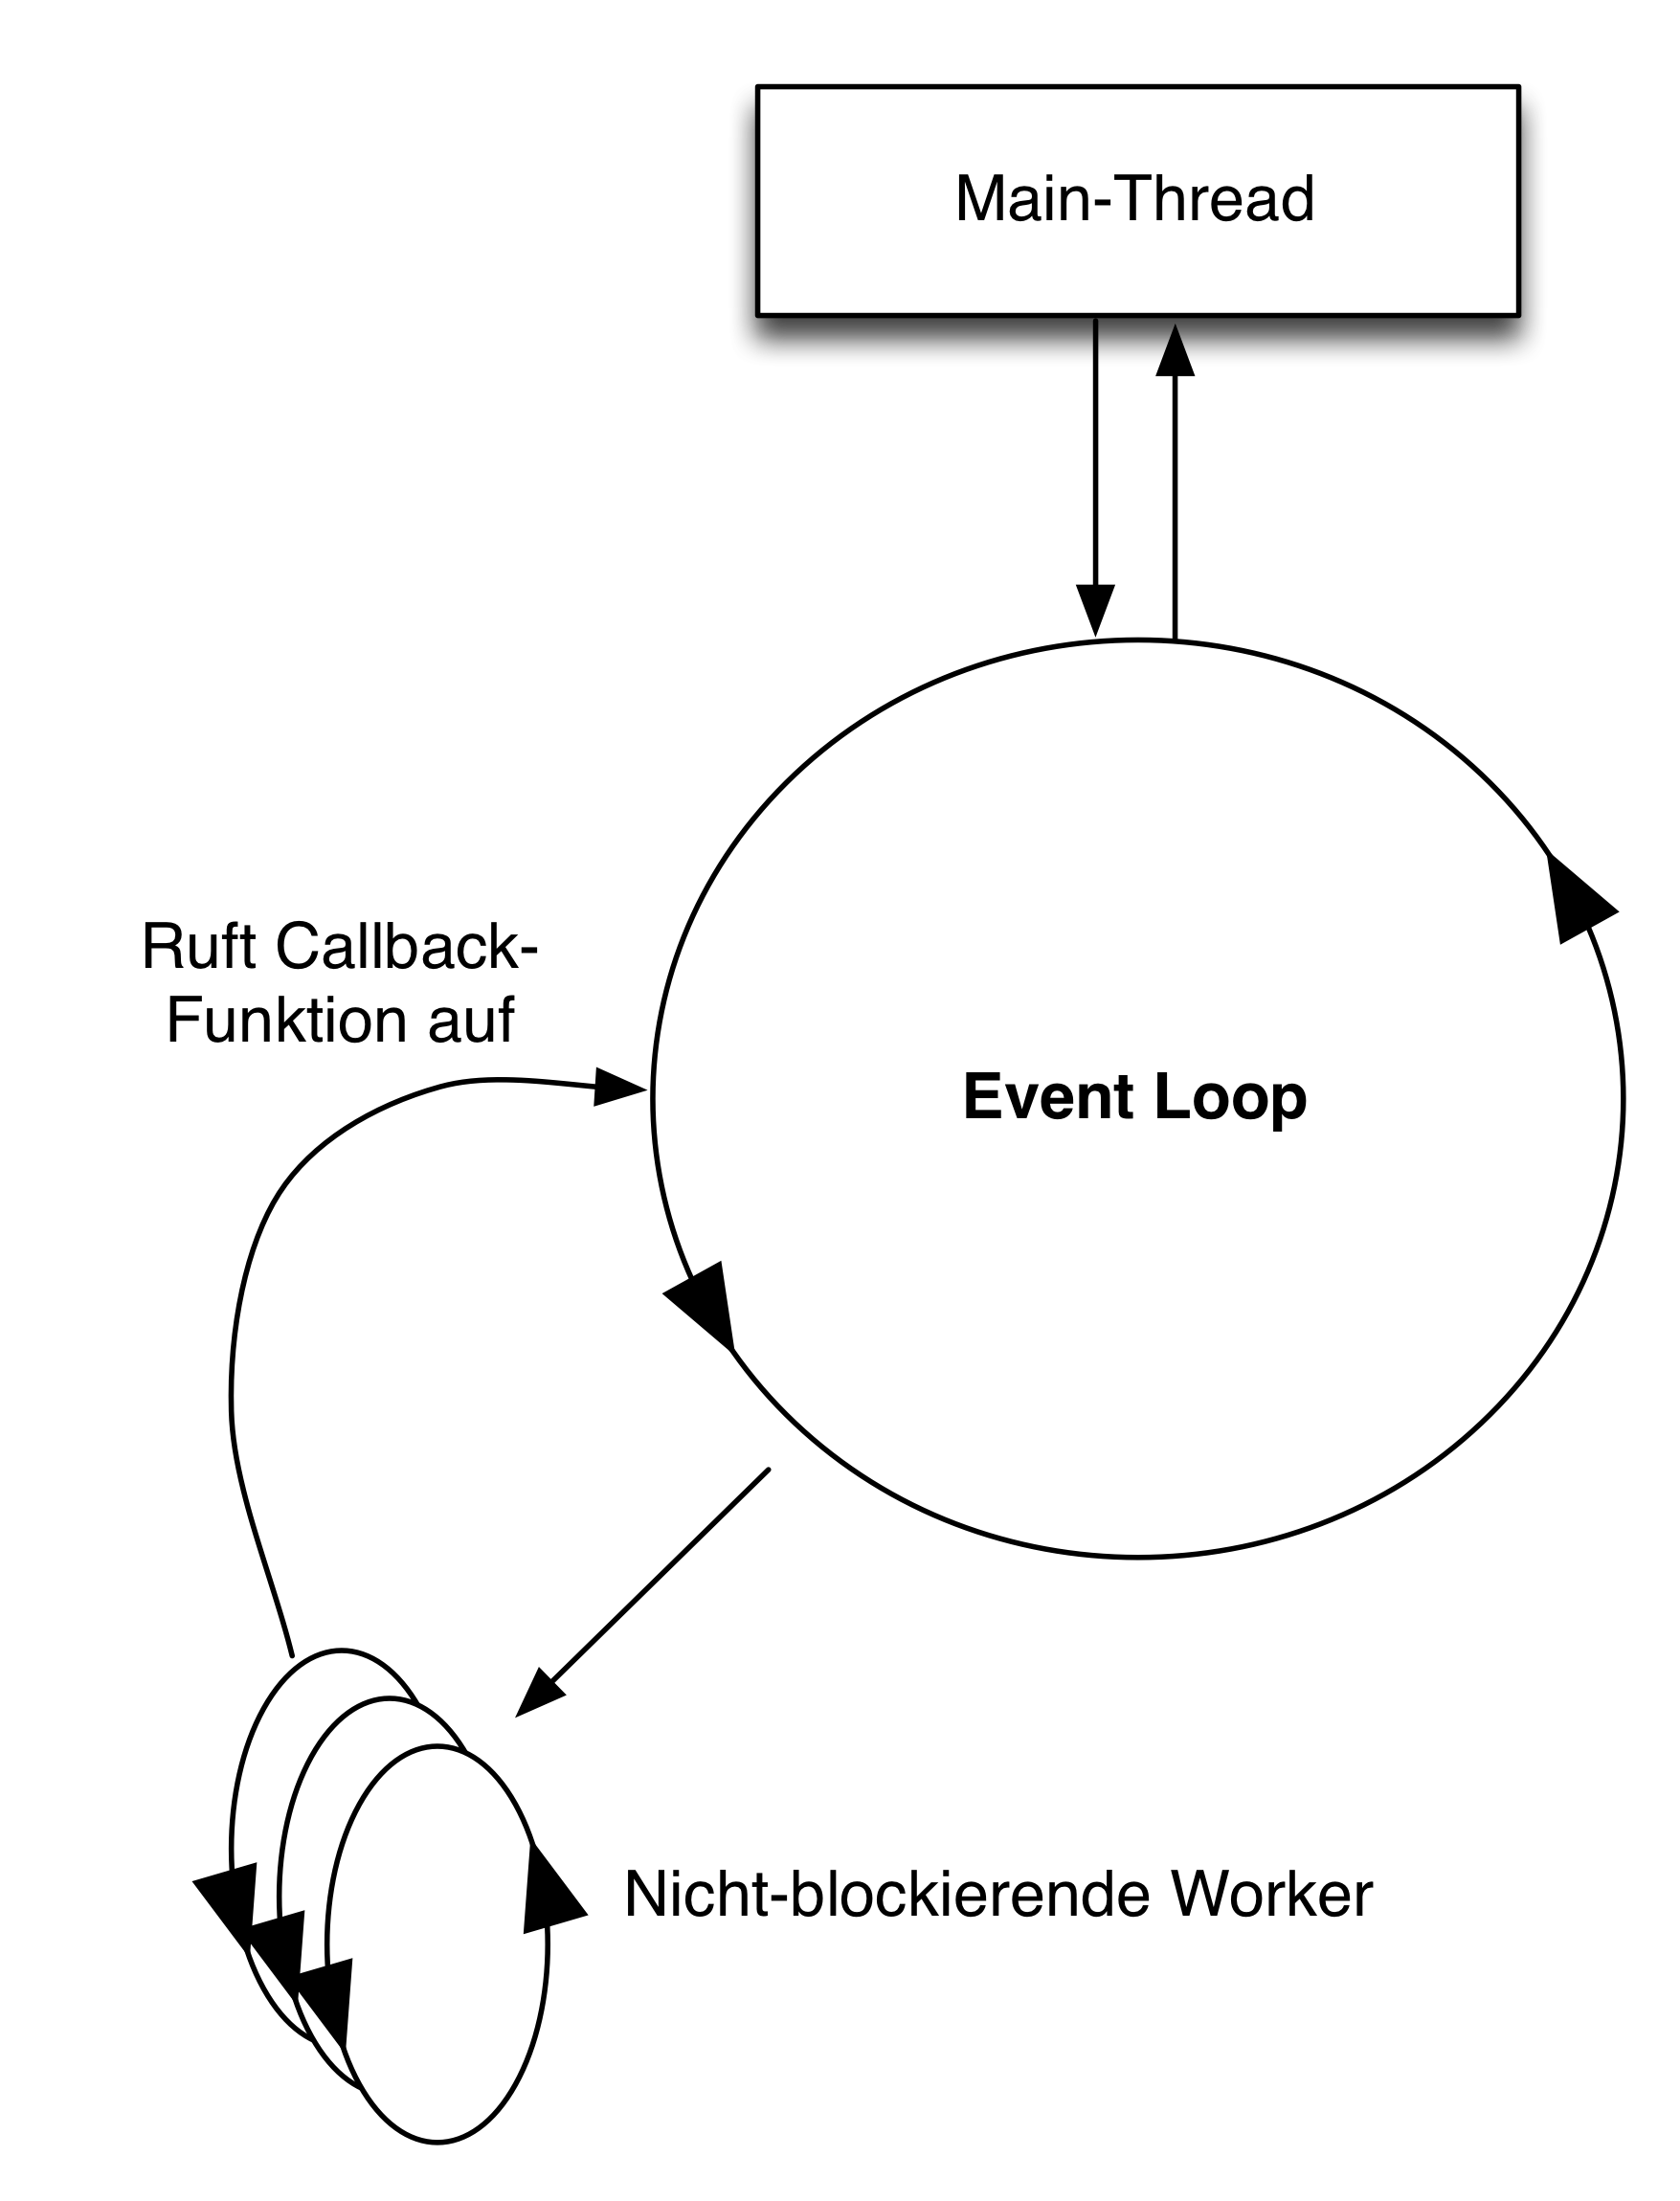
\includegraphics[width=0.4\textwidth]{images/nonblocking.png}
\caption[Event-Loop]{Event-Loop}
\label{img:nonblocking}
\end{figure}
\acresetall
